\section{Literature Review}
This section \colorbox{green}{summarizes} the overview of the two main topics of this research. The first part is the general introduction to active learning and current work on this topic, followed by the review on bayesioan nonparametric models sharing the same structure. 
\newcommand{\argmax}[1]{\underset{#1}{\operatorname{arg}\,\operatorname{max}}\;}
\newcommand{\argmin}[1]{\underset{#1}{\operatorname{arg}\,\operatorname{min}}\;}
\subsection{Background}
Under the background of information explosion, the quick and accurate processing of the data has become an urgent need. However, the traditional classical machine learning shcemes seems not enough to handling this task well, either not time or memory efficient\cite{druck2009active,huang2010active}. Plus, most of the classical algorithms are disigned to perform well on small data set with limited complexity of the model. When introduding to the scenarios dealing with large-scale data set, it may perform unsatisfatory or fail.

Active learning scheme is designed to address the problem by labeling the data explicitly during the training process, with the aim that reach high accuracy using as few labeled data as possible\cite{Prince2004,Settles2010}. Instead of waiting passively for the data to be \colorbox{green}{sent} in for training, it actively choosing the samples based on the prespecified regularization to reach a best evaluation on the current training step. It often take less steps to reach a similar performance than the passive learning methods. 

Also, big data set often contains more complex model\cite{escobar1995bayesian}. A prespecified model assumption will not satisfy the need of big data learning target. This is where bayesian nonparametric models arise. It allows to the model to adapt its complexity to the data and grow as more data are observed\cite{hjort2010bayesian}. The flexibility make it easier to evolve and reach better performance. 

In the following two parts, we will dive into each of this two subproblems.

\subsubsection{Active Learning}
Active learning is under the hypothesis that if the algorithm is allowed to select the data during training process, then the performance could be improved with less training comapred to the one that without choosing process\colorbox{green}{\cite{Settles2010}}.  In most machine learning scenario\cite{Prince2004,huang2010active}, the algorithm need to be trained on hundreds of labeled instances. However, sometimes the labeled data could be very expensive, time-consuming or difficult to collect. 

\begin{figure}[htbp] 
\centering
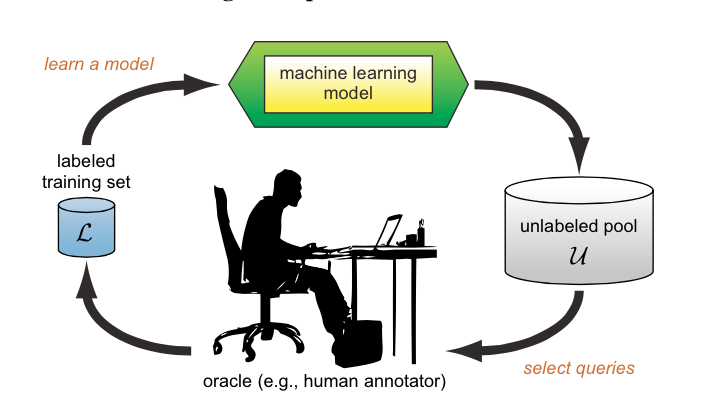
\includegraphics[scale=0.4 ]{activelearning}
\caption{Active Learning System}\label{active_figure}
\end{figure}
Figure.\ref{active_figure} is the general framework of active learning. It mainly consists of two subprocess:sample querying and model training. The model is trained on a small-size data set $\mathcal{L}$, request labels for one or more selected samples then revise the parameters of the model and step into the next loop until certain termination conditions is fulfilled. \colorbox{green}{Figure}\ref{active_comparison}\cite{Settles2010} is the comparison of the learning result on the same data set, with and without active sampling.
\begin{figure}[htb] 
\centering
\subfigure[]
{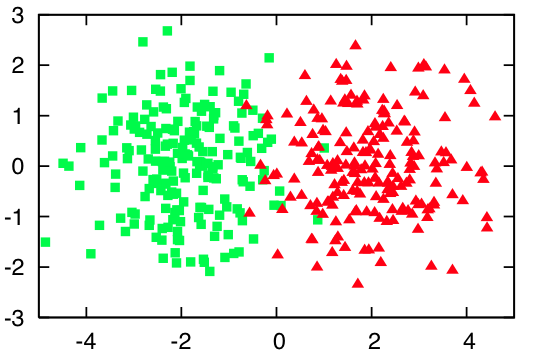
\includegraphics[scale=0.2]{activelearning/demo1}}
\subfigure[]
{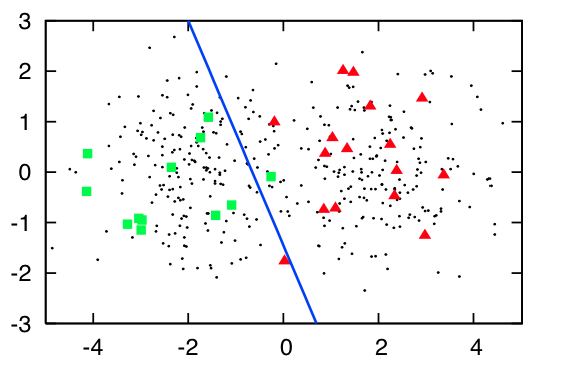
\includegraphics[scale=0.2]{activelearning/demo2}}
\subfigure[]
{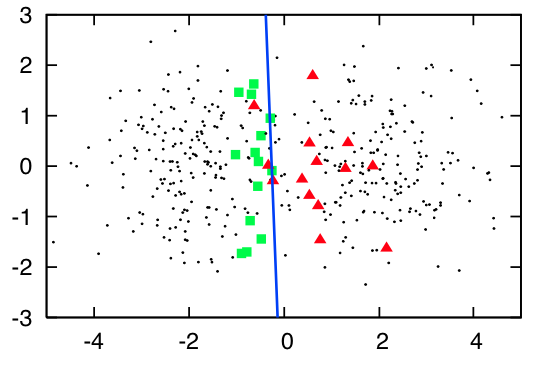
\includegraphics[scale=0.2]{activelearning/demo3}}
\caption{An example of active learning. (a) A toy data set with 400 observations sampled from 2 class Gaussian. (b)A logistic regression model trained with 20 labeled instances from each class. The line is decision boundary(70 \% accuracy) (c) A logistic regression model trained by a total 30 actively selected instances(90\% accuracy)}\label{active_comparison}
\end{figure}
\subsection{Query Strategy Frameworks}
As we mentioned, query strategies lie in the core of active learning framework, by which the candidate instances will be evaluated and the current best one will be selected for the training.  There are t general framework for querying\cite{Settles2010}:
\begin{itemize}
  \item \textbf{Uncertainty Sampling}: selecting the instance about which the model is least certain about. It is oftern used  for binary classification, and the model queries the instance whose posterior probability of being positive is nearest to 0.5, which could also be interpreted in terms of \textbf{information entropy}\cite{dasgupta2008hierarchical}. For multi-class problem, the instance to query is the one whose prediction is the \textit{least confident}\colorbox{green}{\cite{Prince2004}}:
  \begin{equation}
  x_{LC}^{*}=\argmax{x} 1-P_{\theta}(\hat{y}|x)  
  \end{equation}
  where$\hat{y}=\argmax{}_{y}P_{\theta}(y|x)$, or the class label with the highest probability under model $\theta$. However, the least confident way only considers information of the most probable label, resulting in neglecting information about the remaining distribution. Thus a different multi-class uncertainty sampling method called \textit{margin sampling} is proposed:
  \begin{equation}
  x_{M}^{*}=\argmin{x}P_{\theta}(\hat{y_1}|x)-P_{\theta}(\hat{y_2}|x)
  \end{equation}
  where $\hat{y_1} $ and $\hat{y_2}$ are the first two most probable class labels. This method incorporate the posterior of the second most probable label to correct for the shortcoming of least confident strategy.
  \item \textbf{Query-by-Committee}:in this scenario, there is a set of models $M=\{\theta^{(1)},\theta^{(2)},\ldots,\theta^{(c)}\}$ of which each is trained on the same training set. Then each model(called a \textit{committee}) is allowed to vote for the candidate instance. The most informative query is the one they most disagree on. This shceme is to minimizing the version space( Shown in Figure. \ref{vs}\colorbox{green}{\cite{Settles2010}}). 
  \begin{figure}[htbp]
   \centering
   \subfigure[]
   {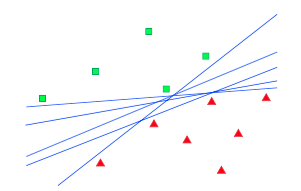
\includegraphics[scale=0.5]{activelearning/vs2}}
   \subfigure[]
   {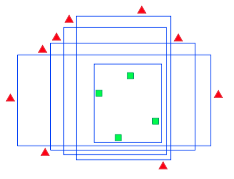
\includegraphics[scale=0.5]{activelearning/vs1}}
   \caption{Version space example(a) Linear and (b)axis -parallel box classifier}
  \end{figure}\label{vs}
  
  There are two common approaches on the measurement of the level of disagreement, among which the first one is \textit{vote entropy}\colorbox{green}{\cite{Settles2010}}
  \begin{equation}
    x_{VE}^{*}=\argmax{x} -\sum\limits_{x}\frac{V(y_i)}{C}\log{\frac{V(y_i)}{C}}  
  \end{equation}
  This could be interpreted in terms of information entropy. Another measure has been proposed is average \textit{Kullback-Leibler(KL) divergence\colorbox{green}{\cite{Prince2004}}}
  \begin{equation}
    x_{KL}^{*}=\argmax{x}\frac{1}{C}\sum\limits_{c=1}^{C}D(P_{\theta^{(c)}}||P_M)
  \end{equation}
  where,
  \begin{equation}
    D(P_{\theta(c)}||P_M)=\sum\limits_{i}P_{\theta^{(c)}}(y_i|x)\log \frac{P_{\theta^{(c)}}(y_i|x)}{P_M(y_i|x)}
  \end{equation}
  As can be seen, $P_M(y_i|x)=\frac{1}{C}\sum^{C}_{c=1}P_{\theta^{(c)}}(y_i|x)$is the \textit{consensus} probability that $y_i$ is the correct label. It also could be reviewed in an information entropy view, i.e  the one with the largest average difference between the label distributions will be regarded as the most informative one. 
  \item \textbf{Expected Model Change}: labelling those points that would most change the current model. It is often used in multi-instance setting and probabilistic sequence models like CRFS. Generally, the EMC model can be applied to any any gradient-based training problem, such as discriminative probalilistic models by measuring the influence of samples\colorbox{green}{\cite{Settles2010}}as the \textbf{Expected Gradient Length}(EGL), and the desired query sample should be the one has the larget magnitude of gradient. Let $\nabla\ell_\theta(\mathcal{L})$ be the gradient of the objective function $\mathcal{L}$ with $\theta$ being the parameter. And let $\nabla\ell_\theta(\mathcal{L}\cup\langle x,y\rangle )$ be the new gradient if complete training instance$\langle x,y \rangle$ is added. As the query function does not know the true label $y$ in advance, the posterior expectation over possible labels will be usedinstead\colorbox{green}{\cite{Settles2010}}:
  \begin{equation}
    x_{EGL}^{*}=\argmax{x}\sum\limits_{i}P_\theta(y_i|x)\|\nabla\mathcal{\ell}_\theta(\mathcal{L}\cup\langle x,y_i\rangle)\|
  \end{equation}
  At each query time, $\|\nabla\ell_\theta(\mathcal{L})\|$ is nearly zero as $\ell$ converged at the previous round, thus we can simply have 
  $\nabla\mathcal{\ell}_\theta(\mathcal{L}\cup\langle x,y_i\rangle)\approx\nabla\mathcal{\ell}_\theta(\langle x,y_i\rangle)$.
  However, this approach could be expensive in computation if it the the labeling set and feature space are both very large.
  \item \textbf{Expected Error Reduction}:labelling those points that would most reduce the model's generalizaion error. This approach is similar to the \textbf{Expected Model Change} except for it measures the generalization error. When the model is trained using $\mathcal{L}\cup\langle x,y \rangle $, the one of which the minimum error on the remaining unlabeled instances will be selected as the query instance. One common way is to minimize the expected $0/1$ loss:
  \begin{equation}
   x_{0/1}^{*}=\argmax{x}\sum\limits_{i}P_\theta(y_i|x)\left (\sum\limits_{u=1}^{U}1- P_{\theta^{+\langle x,y_i\rangle} }(\hat{y}|x^{(u)})\right )
  \end{equation}
  where $P_{\theta^{+\langle x,y_i\rangle}}$ represents the new model with training tuple $\langle x,y_i\rangle$ added to trainging set $\mathcal{L}$. Still the true label remains unknown, so we go through all possible labels. 
  \item \textbf{Random Sampling}: This is a random sampling process, often used as a test base for other algorithms.
\end{itemize}

With the goal of labeling the most informative instances to achieve high prediction accura- cies with minimum cost, active learning is a continuously growing area in machine learning research. We have put the emphasis on the design of  query strategies for instance selection criteria. In practical problem, different querying functions could be used under different settings according the type of the problem. 
In summary, the sampling process could be concluded to a 'selecting the current best' procedure which implies that each step contains a massive comparison process. Instead of sampling on the whole unlabeled data set, research on just a subset of it is believed to lead to a more economical learning process\cite{Settles2010,cohn1994improving,meyers1993promoting}.
That is the reason why we are trying to introduce Baysian nonparametric Models(section \ref{bnp}) into the framework of active learning.


\subsubsection{Bayesian Nonparametric Models}\label{bnp}
In this section, we will briefly describe another topic in this research, the baysian nonparametric models.
Most machine learning problem is targeted to learn a set of parameters describing the model from training data set. This sort of learning is often evaluated in two terms, with the first one being how well the model fits the data, expressed as accuracy or squared error, and the second one being a complexity penalty(favoring simpler models)\cite{gershman2012tutorial,escobar1995bayesian}, also referred to as Ocam's Razor. In practical problem, the model complexity is hard to evaluate. Improper model complexity will lead to over-fitting or under-fitting\cite{gershman2012tutorial,muller2004nonparametric}, which will then affect the model generalization, i.e to be applied to practical use. Although through rigid training, desirable models could be trained but this is basically a trial and error process\cite{hjort2010bayesian}. That is the movivation of discovering adaptive model complexity selection methods, among which Bayesian Nonparametric Method is the most widely used.

Bayesian nonparametric models provide a different way to address the problem. Instead of comparin gmodels that vary in complexity, it fits a single model that can adapt its complexity to the data. It is opposed to parametric schemes which uses a fixed number of parameters. For example, a parametric approach to density estimation would be to fit a Gaussian or a mixture of a fixed number of Gaussians by maximum likelihood\cite{walker1999bayesian,andrews2002support}. while in a nonparametric settings, it is often using Parzen window centering  a Gaussian distribution at each observation to estimate the parameters. 

Nonparametric methods is very popular in classical (non-Bayesian) statistics. They often perform impressively in applications and the theoretical properties have been introduced to a wide range of models, each of which will give a brief introduction below:
\begin{enumerate}
 \item \textbf{Clustering with mixture models}
  
  In BNP framework, the clustering problem could be addressed with estimating both the number of components and parameters of each individual mixture component concurrently\cite{gershman2012tutorial,escobar1995bayesian}. The model is often expressed as $p(x)=\sum_{k=1}^{K}\pi_kp(x|\theta_k)$, with $\pi_k$being the mixing proportion associating with the parameters $\theta_k$ in component $k$. The density could be expressed as $p(x)=\int p(x|\theta)G(\theta)d\theta, G=\sum_{k=1}^{K}\pi_k\delta_{\theta_k}$, $G$ is a discrete mixing distribution and $\delta_k$ is a Dirac distribution centered at $\theta$. BNP mixtures use a mixing distributions consisting of a countably infinite number of atoms $G=\sum_{k=1}^{\infty}\pi_k\delta_{\theta_k}$ allowing for mixing with an infinite number of components. The Bayesian requires a prior over the mixing distribution $G$, mostly Dirichlet process, expressed as $DP(\alpha,H)$ with $\alpha>0$ being the concentration parameter and a base distribution $H$ being prior over sistributions. Thus for any partition $A_1,\cdots,A_m$ of the parameter space, the random vectom$(G(A_1),\cdots,G(A_m))$ is Dirichlet distributed. If the partition is over integars, the DP is also called Chinese Restaurant Process(CRP).
 \item \textbf{Nonlinear Regression}
 
 Parametric approaches to adress the regression problem is to parameterize the function using a set of finite number of parameters and estimate their values from the data directly. However, in a Bayesian nonparametric framework, a prior distribution over continuous functions if defined, called a Gaussin Process(GP)\cite{rasmussen2006gaussian}. It is a distribution on an infinite collection of random variables $X_t$, and for any finite subsets$X_{t_1},\cdots,X_{t_m}$, the joint distribution is a multivariate Gaussian. The Gaussian process posterior is a distribution on functions given the training set. 
 
 \item \textbf{Density Estimation}
 
 In BNP, density estimation problem could be addressed by defining a prior on densities or distributions, and the distributions should be smooth on the empirical density\cite{lo1984class}. While DP can generate discrete distributions only, it is not very useful under this context. Instead we use DP mixture models and Polya trees as the prior distribution\cite{ghosal1999posterior}. 
\end{enumerate}

When the model is selected, another important issue is the inference in BNP. There are often two aspects concerning this issue: the analytic tractability of posterior for the stochastic process embedded in BNP model and practical inference methods\cite{walker1999bayesian,muller2004nonparametric}. For the analytic way, a conjugate prior is used to guarantee that an closed-form posterior is feasible. But for some distributions it would be difficult to find a conjugate prior. BNP often contains Dirichlet process or Gaussian process. These processes have infinite number of dimensions and naive algorithm is infeasible. However, they generally have analytically tractable posteriors, and most dimensions could be directly integrated out. For the remaining dimensions, we can handle them by the usual inference methods in parametric modeling, such as Markov Chain Monte Carlo, sequential Monte Carlo, Variational Inference and message passing algorithms like expectation propagation\cite{hjort2010bayesian,muller2004nonparametric}. And the specific choice of inference methods is based on the actual problem, with accuracy and efficiency taking into consideration. 

Though the powerful modelling ability of BNP model, the close-form solution to it is ofter intractable due to the integeration on functions that could not be integrated. As an alternative, Sampling Methods is designed to select a statistical sample to approximate a hard combinatorial problem. This approach is based on Law of large numbers in statistical theory\cite{ASB:8937274}. Often, when the number of samples reaches infinity, the estimation is believe to be the acceptable value of true variable with an bearable error. However, MCMC requires a large -scale sampling process and all the samples will be stored for the estimation of unknowns. 

As in BNP modelsthe main drawback constraining the BNP model is the efficiency , which is also the bottleneck of the nonparametric methods family\cite{hollander2013nonparametric}. Although sampling method such as MCMC provide a plausible way for the parameter estimation, when the data size increases this will lead to disastrous on need of cost\cite{ghosh1982nonparametric}.
\subsection{Summary}

In this section, we briefly review the two main topic in this proposed research. Generally, Active Learning is an important subsection in machine learning and very promising since it aims to address the bottleneck due to insufficient training instances. We exploited the general problem and main aspects in active learning. And for Bayesian Nonparametric models, it tries to overcome the shortcomings in traditional parametric methods and the flexibility allows for adaption of the model to fit the data,  this is especially important on the model generalization. 

By the analysis in this section, these two branches could be complementary to each other if these are used under the same famework and form a loop of feedback for each other's training stage. BNP model will cluster the dataset adaptively and recommend the most representative sample for active learning. Similarly, active learning will in returen recommend the BNP model which set of point is more preferred which will guide the BNP model updating. 

This close-loop framework is the one we are desired to develop, the performance of similar frameworks in the other area has been proved\cite{zhang2011close}.